\documentclass[12pt]{article}

% Some typesetting decisions
\usepackage[utf8]{inputenc}
\usepackage{graphicx}
\usepackage{verbatim}
\usepackage{subcaption}
\usepackage{amsmath, amssymb}
\usepackage{mwe}
\usepackage[title]{appendix}
\usepackage{babel}
\usepackage{todonotes}

% Typesetting and basic formatting. 
% This PDF is made to be read on-screen,
% so we use large fonts and little margin
\usepackage[margin=30mm]{geometry}
\usepackage{setspace}
\setstretch{1.1}
\setlength{\parindent}{0pt}
\setlength{\parskip}{12pt}
\frenchspacing 
\sloppy


% Links
\usepackage{xcolor}
\usepackage{hyperref}
\hypersetup{colorlinks,linkcolor={blue!50!black},citecolor={blue!50!black}, urlcolor={red!50!black}}  
% This one is for demo-purposes only, don't use it in your submission ;) 
\usepackage{blindtext}

% Citation with natbib: 
% Use \citet{} and \citep{} only, not \cite{}
\usepackage{natbib}
\bibliographystyle{abbrvnat}

\DeclareMathOperator*{\argmax}{arg\,max}


%%%%%%%%%%%%%%%%%%%%%%%%%%%%%%%%%%%%%%%%%%%%%%%%%%%%%%%%%%%%%%%%%%%%%%%%%%%%%%%%%%%%%%%%%%%%%%%
% non template commands

\title{\vskip-3em \bf 
    Climate Network Communities for Precipitation Data
    }
\author{
    A Summary Written by Johannes Schulz and Adrian Stock \\
    \texttt{johannes.schulz@student.uni-tuebingen.de} \\
    \texttt{adrian.stock@student.uni-tuebingen.de}
}
\date{\it Machine Learning Approaches in Climate Science\\Summer Term 2021}


\begin{document}

\maketitle
\thispagestyle{empty}

\newpage
\pagenumbering{arabic}

\begin{comment}
    \begin{abstract}\vskip-1.5em \noindent
        We looked at different papers that detected network communities on climate data \citep*{community_structure,complex,exploration}.
        To implement the stochastic block model, we used the pysbm package \citep{sbms}.
    \end{abstract}
\end{comment}

\begin{section}{Introduction}
In recent years, it has become more and more obvious that the consequences of climate change are making themselves felt. To deal with the increasingly frequent extreme weather phenomena, we need accurate and reliable models of the weather's dynamics and the underlying climate system. \\
In this work, we present an algorithm to detect network communities. Network communities are regions that show similar behaviour in their dynamics. We have a look at precipitation data from the ERA5 dataset provided by Copernicus \citep{hersbach2019era5} over Western Europe (75N-35Nx15W-40E, Fig. \ref{fig:region_covered}) with a spatial resolution of 0.25°. Furthermore, each point in space corresponds to a series of monthly precipitation values from 01.01.1979 - 01.04.2021. This leads to a dataset with 161 x 221 data points and a time series of length 507 per data point. For a lack of computational resources, the data set is downsampled to a size of 33 x 45 x 507. In the following, we first generate a graph representing Western Europe. Afterwards, we use Stochastic Block Modelling to infer network communities in this graph. At the end, the results of the experiments are presented and related to the North Atlantic Oscillation (NAO). This is a well-researched biphasic weather phenomena that is caused by high pressure regions over the Azores. In the NAO positive phase the weather in Northern Europe is rather wet while being dry in the south of Europe. The opposite is true in the NAO negative phase.
\end{section}

\begin{section}{Graph Generation}
A graph $G=(V,E)$ is represented by a tuple of nodes $V$ and edges $E$.
In our case, $V$ contains all grid cells over Western Europe that are present in our data set. 
Each grid cell corresponds to a location for which we have a time series measurement of precipitation data. 
As we want to detect regions with similar behavior, we draw edges between two nodes/locations if their corresponding time series are sufficiently, i.e. statistically significantly correlated.
As a measure of correlation between two time series $t_1$ and $t_2$, we use the pearson correlation coefficient: 
\begin{equation}
    \rho_{t_1, t_2} = \frac{\text{cov}(t_1, t_2)}{\sigma_{t_1}\cdot \sigma_{t_2}}
\end{equation}
Statistical significance is a concept stemming from hypothesis testing.
    %Suppose for the moment that the measurements in a single time series $t$ are $i.i.d.$.
    %Concretely, $t \sim \prod\limits_{i=1}^N p(t_i)$. In practice this assumption is not justified, as the %weather at the present moment depends on the weather in the past (section \ref{autocorr}). 

\begin{subsection}{Hypothesis Testing}
We start by considering two different hypotheses.
\begin{itemize}
    \item $H_0$ := $t_1$ and $t_2$ are uncorrelated, i.e. $p(t_1, t_2) = p_1(t_1) \cdot p_2(t_2)$
    \item $H_1$ := $t_1$ and $t_2$ are correlated
\end{itemize}
Additionally, we need a test statistic $T(t_1, t_2) = \rho_{t_1, t_2}$, in our case the correlation coefficient.
Instead of thinking about $p(H_1)$ directly, which is what we are interested in, hypothesis testing considers $p(T(t_1, t_2) \mid H_0)$.
In other words: How likely is the correlation we observe under the assumption that the time series are actually not correlated. For a given significance level $\alpha$, two time time series $t_1$ and $t_2$ are said to have a statistically significant correlation if $p(T(t_1, t_2) \mid H_0) < \alpha$. In that case we reject the null hypothesis $H_0$ and accept $H_1$.
Figure \ref{fig:hypothesis_testing} shows an approximate distribution ($N = 100000$) of the test statistic (correlation coefficient) under the null hypothesis as well as the rejection region for $\alpha = 0.001$. 
As we preprocessed our data to have mean 0 and variance 1, we sample $t \sim \mathcal{N}(t;0,1)$ from a normal distribution that shares the same properties.
\end{subsection}

\subsection{Autocorrelation}
Looking at figure \ref{fig:correlations}, we can observe that our hypothesis test would only reject the null hypothesis in about 50$\%$ of the cases. This seems wrong as it indicates that on average each location in Western Europe is significantly correlated with about $50\%$ of all other locations.
The reason for that can be found in the autocorrelation (i.e. the correlation of a timeseries with its past), which is quite similar for all locations in Western Europe. 
An example of that are seasonal shifts of the weather which are the same in all of europe.
Therefore, the total correlation $\textbf{c}_\text{total}$ can be decomposed into the "true" correlation
 $\textbf{c}_\text{true}$ and the correlation $\textbf{c}_\text{autocorr}$ which is caused by a similar autocorrelation structure of the two time series. 
\begin{equation}
    \textbf{c}_\text{total} = \textbf{c}_\text{true} + \textbf{c}_\text{autocorr}
\end{equation}
To detect $\textbf{c}_\text{autocorr}(t_1,t_2)$, we employ an algorithm, implemented by \citeauthor{rand_perm_alg}, that is able to randomly permute a timeseries while keeping the autocorrelation intact \citep{rand_perm}.
Computing the correlation between $t_1$ and $t_2^{perm}$ for a sufficiently high sample size gives us an approximation for $\mathbb{E}[\textbf{c}_\text{autocorr}(t_1, t_2)]$ as there is no true correlation between $t_1$ and a random permutation of $t_2$ ($\mathbb{E}[\textbf{c}_\text{true}(t_1,t_2^{perm})] = 0$).
As, we only want to compute significance based on $\textbf{c}_{true}$, our rejection region is shifted by $\mathbb{E}[\textbf{c}_\text{autocorr}(t_1, t_2)]$ (\ref{fig:correlations}).
Nevertheless there were still too many statistically significant positive correlations, so we shifted our rejection region for positive correlations again to make our results more comprehensible. 
The final graphs are shown in figures \ref{fig:positive_correlations} and \ref{fig:negative_correlations}.

\end{section}

\begin{section}{Community Detection}
Given that we have our graphs for positive and negative correlations respectively, we now want to detect communities, i.e. regions that share similiar characteristics. To do so, we use Stochastic Block Models (SBM) \citep{sbms}, as they provide a probabilistic inference method based on solid theoretical foundations, while being comparatively simple. 

\begin{subsection}{Stochastic Block Modelling}
SBMs are based on two main assumptions: 
\begin{itemize}
    \item each node $i$ belongs to exactly one community $q_i \in \{1, \dots, K\}$
    \item Stochastic Equivalence: $p((i,j) \in E) = f(q_i, q_j) = C_{q_i, q_j}$
\end{itemize}
Stochastic equivalence tells us that the probability of a connection between two nodes only depends on the communities each node belongs to.
While being appropriate for our model, this is not generally the case (think about people in a social network).
Based on these two assumptions we can create a generative model, that is based on $\Theta = \{q \in \mathbb{R}^n, C \in \mathbb{R}^{K\times K} \}$.
Inference can now be performed using ML estimation: Given a graph in from of an adjacency matrix $A \in \mathbb{R}^{N \times N}$, we want to find parameters $\Theta^*$, that maximize the probability of observing $A$: 
\begin{equation}
    \Theta^* = \argmax\limits_\Theta \mathcal{L}(\Theta) = \argmax\limits_\Theta P(A\mid \Theta)
\end{equation}
While $C^*$ can be analytically inferred, $q^*$ has to be approximated as it is not tractable. 
Karrer inference \citep{karrer_inference} is a greedy MCMC algorithm that starts with a random initial configuration for $q$ and always ends up in a local maximum. 
We use this method for different initializations and choose $q^*$ as the one that gives us the highest likelihood.
\end{subsection}

As $K$, i.e. the number of communities, does not appear in the set of parameters for the SBM, it has to be chosen as a hyperparameter.
To do that, we use a regularized version of the BIC (Bayesian Information Criterion) score, such that the best $k$ is the optimal trade-off between accuracy (log likelihood) and complexity (number of parameters):
\begin{equation}
    \text{BIC} = \log\mathcal{L}(\Theta) + \lambda \cdot |\Theta|
\end{equation}
For regularization parameter $\lambda=1000$, we end up with $k=5$ and $k=4$ respectively.
Figures \ref{fig:communities_positive_correlations} and \ref{fig:communities_negative_correlations} show the final resulting communities.


\end{section}

\section{Conclusion}

As we can see in Fig. \ref{fig:communities_positive_correlations} the presented algorithm is able to infer meaningful communities (the Mediterranean area, Scandinavia, ...). Moreover, the communities in green and yellow directly relate to the NAO, as both are densely connected in themselves but not connected to another. This observation is further validated by Fig. \ref{fig:communities_negative_correlations}. Here we can see points in northern Europe (drawn in blue) that highly anti-correlate the south of Europe (points drawn in green).
However, the experiments also give results that cannot be explained by NAO. It is noticable that there are only a few points in the north but many points in the south in Fig. \ref{fig:communities_negative_correlations}. Furthermore, the area around the United Kingdoms is one community (drawn in black, Fig. \ref{fig:communities_positive_correlations}). Both observations could be used as a starting point for future research.\\
Ultimately, we showed that Climate Networks are powerful models that can give reasonable results with information about only one climate variable (i.e. precipitation). Including additional variables, such as temperature or pressure, should enhance the quality of the results. We believe that the modelling of network communities could play a crucial part in researching and understanding weather dynamics in the future.


\bibliography{bibfile}

\newpage

\appendix
\begin{Huge}
    \textbf{\appendixname}
\end{Huge}
\newline
\section{Figures}


\begin{figure}[ht]
    \centering
    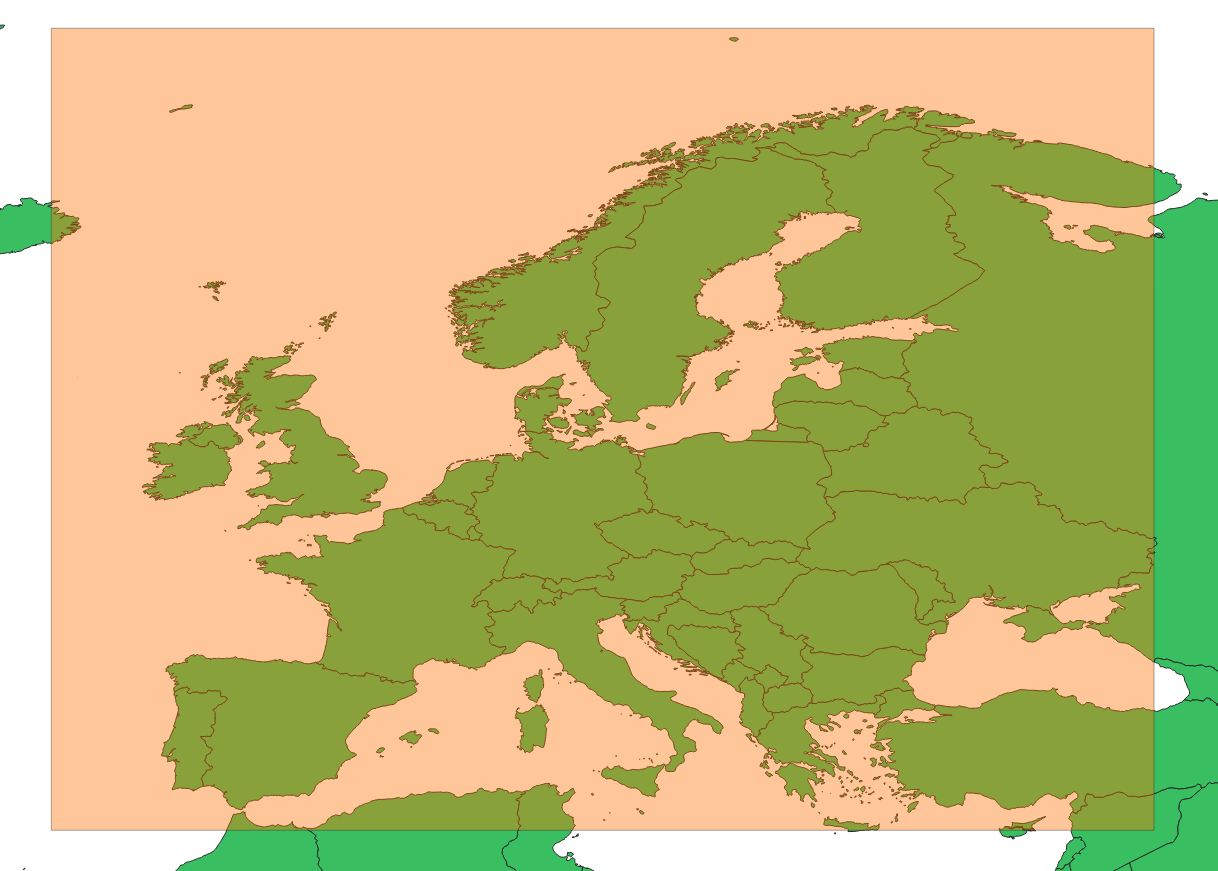
\includegraphics[width=\linewidth] {graphics/considered_region_western_europe.png}
    \caption{Region covered in the experiments}
    \label{fig:region_covered}
\end{figure}

\begin{figure}[ht]
    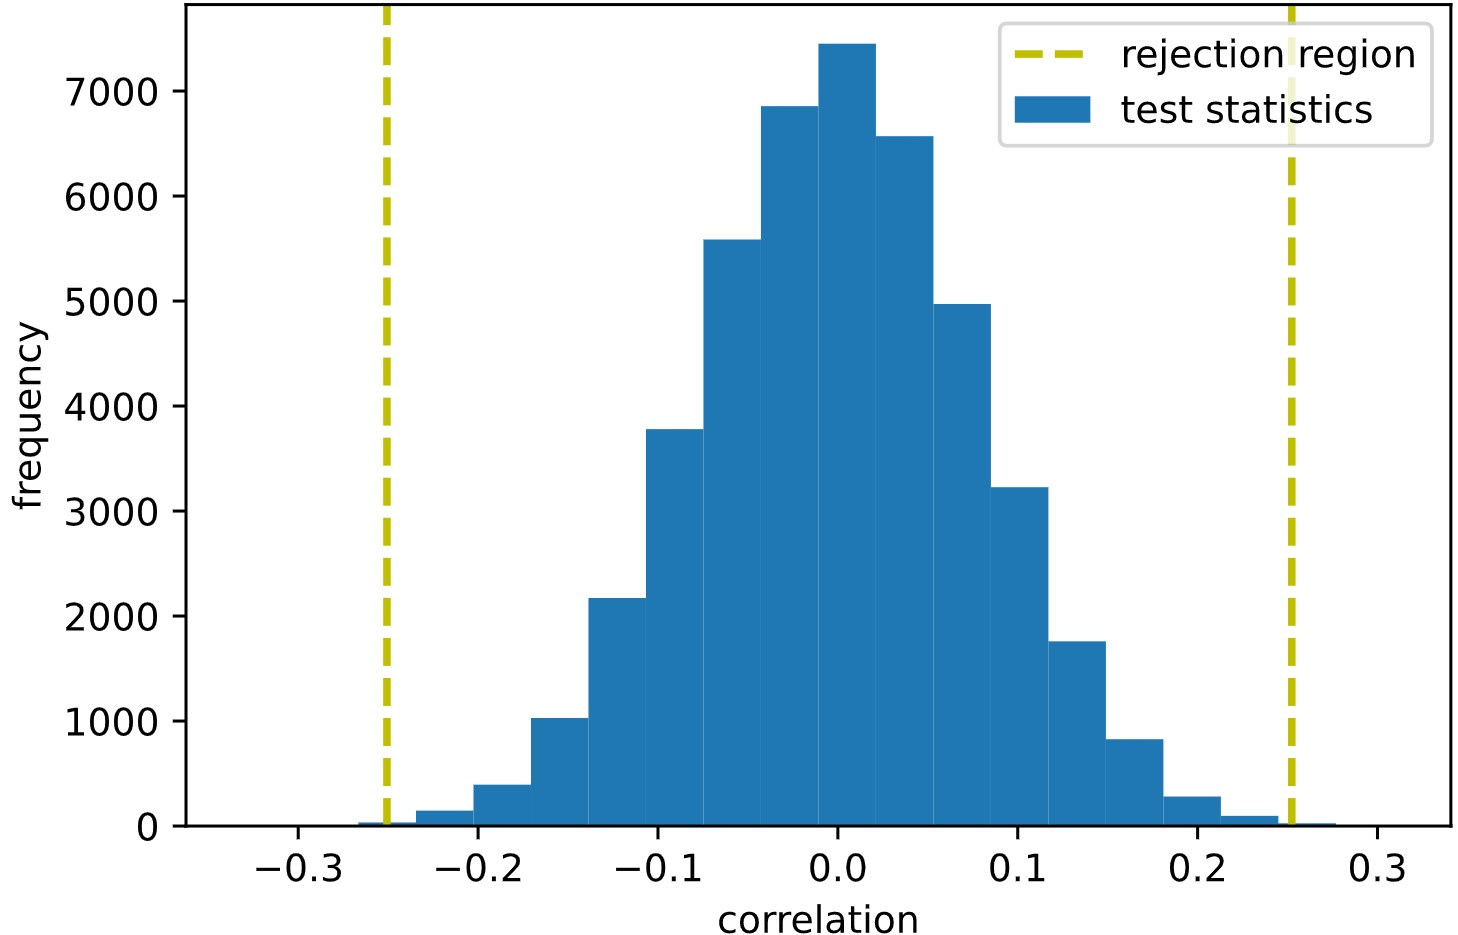
\includegraphics[width=\linewidth] {graphics/hypothesis_testing.jpg}
    \caption{Correlation coefficient under $H_0$}
    \label{fig:hypothesis_testing}
\end{figure}


\begin{figure}[ht]
    \hspace{-1cm}
    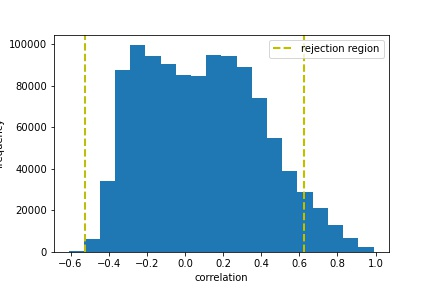
\includegraphics[width=1.2\linewidth] {graphics/correlations.jpg}
    \caption{Observed Correlations}
    \label{fig:correlations}
\end{figure}
        
        
\begin{figure}[ht]
    \centering
    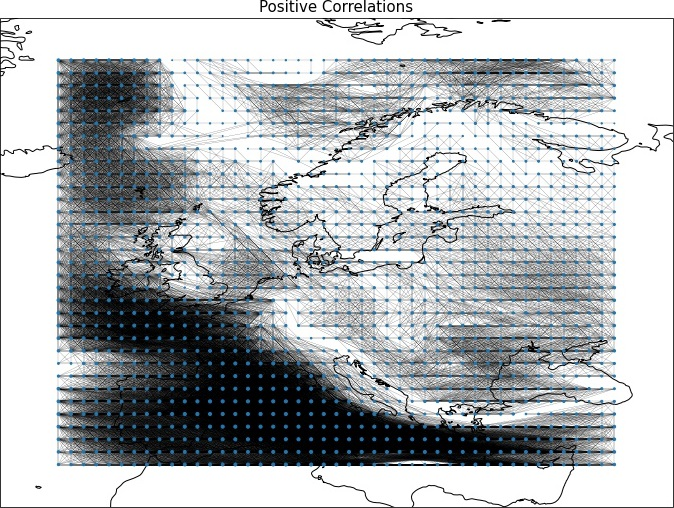
\includegraphics[width=\linewidth] {graphics/positive_correlations.jpg}
    \caption{Positive Correlations}
    \label{fig:positive_correlations}
\end{figure}

\begin{figure}[ht]
    \centering
    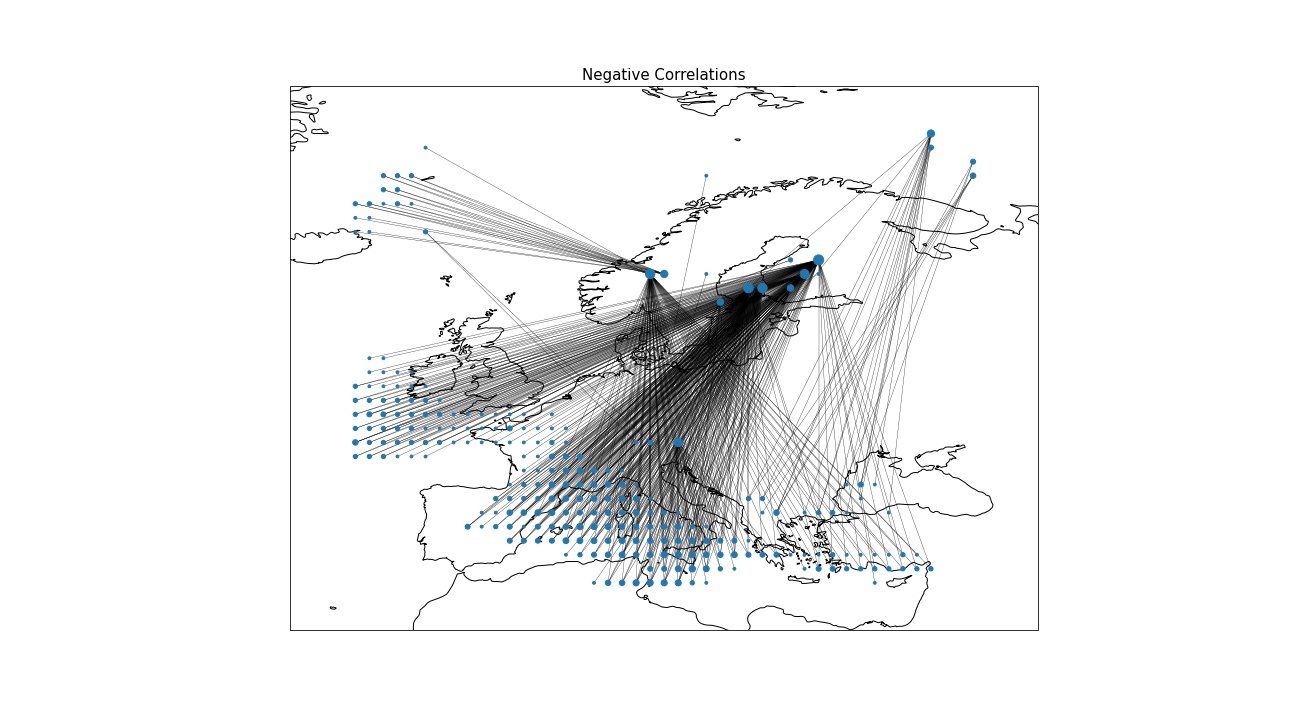
\includegraphics[width=\linewidth] {graphics/negative_correlations.jpg}
    \caption{Negative Correlations}
    \label{fig:negative_correlations}
\end{figure}

\begin{figure}[ht]
    \centering
    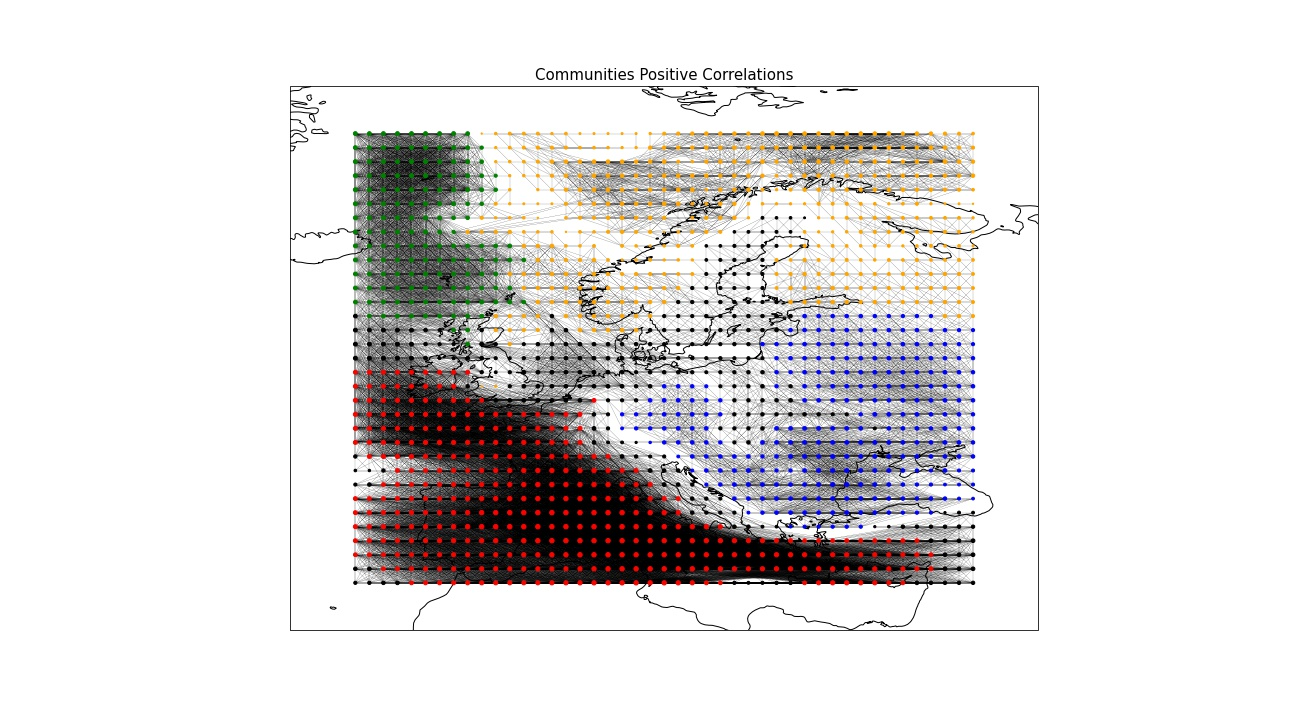
\includegraphics[width=\linewidth] {graphics/communities_positive_correlations.jpg}
    \caption{Communities positive Correlations}
    \label{fig:communities_positive_correlations}
\end{figure}

\begin{figure}[ht]
    \centering
    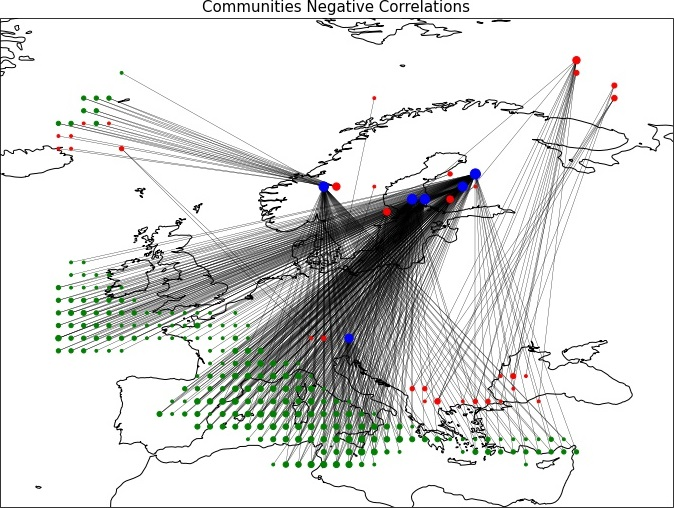
\includegraphics[width=\linewidth] {graphics/communities_negative_correlations.jpg}
    \caption{Communities negative Correlations}
    \label{fig:communities_negative_correlations}
\end{figure}

\begin{figure}[ht]
    \centering
    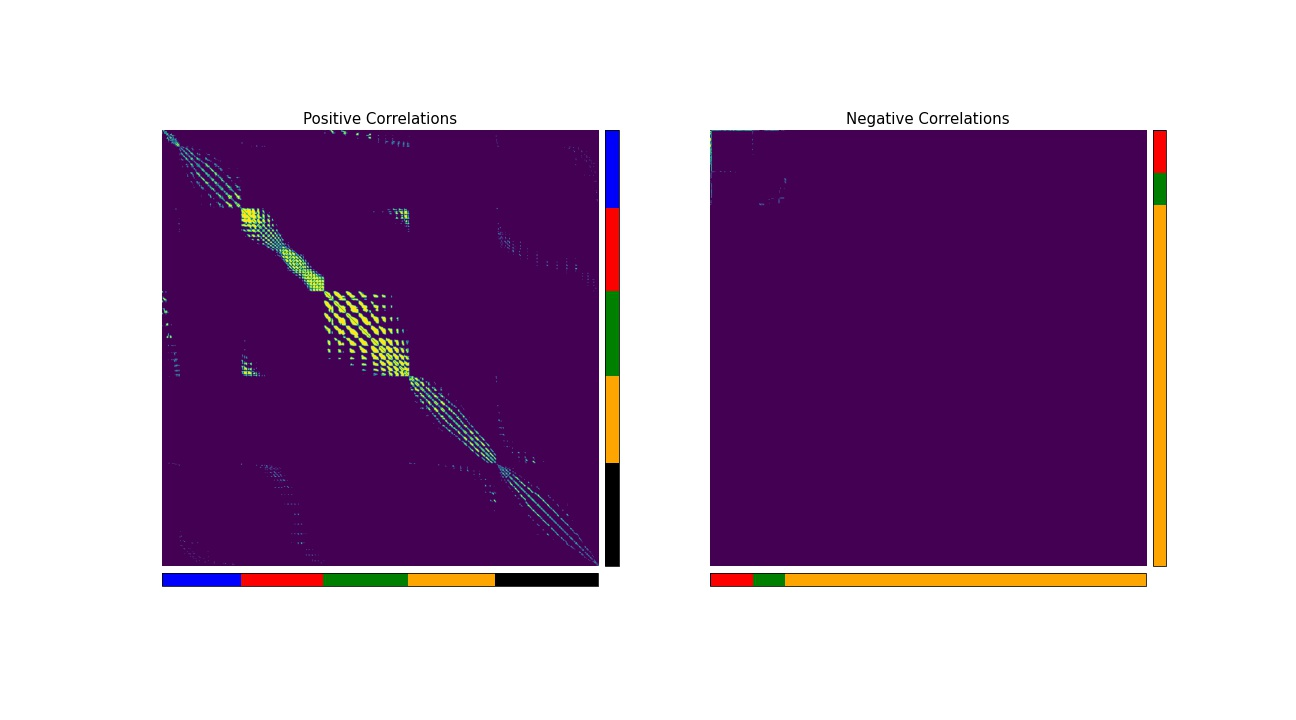
\includegraphics[width=\linewidth] {graphics/adjacency_matrices.jpg}
    \caption{Adjacency matrix for communities on positive correlations graph}
    \label{fig:adjacency_matrices}
\end{figure}

\end{document}